\clearpage

\section{Opaque with 1+1 Protection}
In this case study we focus on the opaque case with 1 + 1 protection.
The opaque transport mode performs OEO (optical-electric-optical) conversions on each intermediate node from the source to the destination node.
One advantage of this mode of transport is that it eliminates accumulation of physical impairments, and allows optimum grooming by performing grooming at each node.

\subsection{Physical Network Topology}
\begin{tcolorbox}	
\begin{tabular}{p{2.75cm} p{0.2cm} p{10.5cm}} 	
\textbf{Student Name}  &:& Tiago Esteves    (October 03, 2017 - )\\
\textbf{Goal}          &:& Implement the dimensioning of optical networks in the opaque transport mode.
\end{tabular}
\end{tcolorbox}
\vspace{-5pt}

\subsubsection{Reference Network}
In the figure below we ca see that our reference network consists of 6 nodes and 8 Bidirectional links.
The average length of the links was chosen so that the following calculations are more simplistic, for this was created a matrix of distances between the respective nodes.
Finally, ODU's matrices were also created to be able to determine the total traffic used in each scenario.

\begin{figure}[h!]
\centering
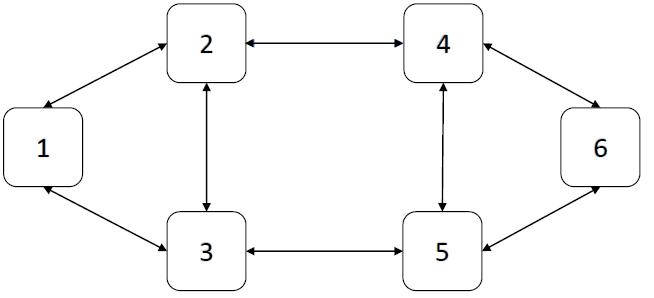
\includegraphics[width=\textwidth]{RedeTeste}
\caption{Physical topology of the reference network.}
\end{figure}

The distance matrix is the same for the two scenarios but the ODU's matrices are not.
In this way only the matrices for the case of low traffic are elucidated, being that in the case of a high traffic it is only necessary to multiply these matrices by the value 10.

\[
Dist=
  \begin{bmatrix}
    0 & 500 & 500 & 0 & 0 & 0 \\
    500 & 0 & 400 & 500 & 0 & 0 \\
    500 & 400 & 0 & 0 & 500 & 0 \\
    0 & 500 & 0 & 0 & 600 & 450 \\
    0 & 0 & 500 & 600 & 0 & 550 \\
    0 & 0 & 0 & 450 & 550 & 0
  \end{bmatrix}
\]

\[
ODU0=
  \begin{bmatrix}
    0 & 5 & 1 & 3 & 1 & 3 \\
    5 & 0 & 0 & 1 & 5 & 0 \\
    1 & 0 & 0 & 1 & 4 & 1 \\
    3 & 1 & 1 & 0 & 1 & 0 \\
    1 & 5 & 4 & 1 & 0 & 3 \\
    3 & 0 & 1 & 1 & 3 & 0
  \end{bmatrix}
\quad ODU1=
  \begin{bmatrix}
    0 & 2 & 4 & 2 & 0 & 5 \\
    2 & 0 & 0 & 3 & 1 & 1 \\
    4 & 0 & 0 & 1 & 1 & 0 \\
    3 & 3 & 1 & 0 & 1 & 3 \\
    0 & 1 & 1 & 1 & 0 & 1 \\
    5 & 1 & 0 & 3 & 1 & 0
  \end{bmatrix}
\quad ODU2=
  \begin{bmatrix}
    0 & 1 & 1 & 1 & 0 & 0 \\
    1 & 0 & 0 & 0 & 1 & 0 \\
    1 & 0 & 0 & 1 & 1 & 0 \\
    1 & 0 & 1 & 0 & 1 & 0 \\
    0 & 1 & 1 & 1 & 0 & 1 \\
    0 & 0 & 0 & 0 & 1 & 0
  \end{bmatrix}
\]
\[
ODU3=
  \begin{bmatrix}
    0 & 0 & 0 & 0 & 0 & 0 \\
    0 & 0 & 1 & 0 & 0 & 1 \\
    0 & 1 & 0 & 0 & 1 & 0 \\
    0 & 0 & 0 & 0 & 0 & 0 \\
    0 & 0 & 1 & 0 & 0 & 0 \\
    0 & 1 & 0 & 0 & 0 & 0
  \end{bmatrix}
\qquad ODU4=
  \begin{bmatrix}
    0 & 0 & 0 & 0 & 0 & 0 \\
    0 & 0 & 0 & 0 & 0 & 1 \\
    0 & 0 & 0 & 0 & 0 & 0 \\
    0 & 0 & 0 & 0 & 0 & 0 \\
    0 & 0 & 0 & 0 & 0 & 1 \\
    0 & 1 & 0 & 0 & 1 & 0
  \end{bmatrix}
\]

Through these ODU's we can calculate total network traffic for the low traffic scenario:\\
$T_1^0$ = 60x1.25 = 75 Gbits/s \qquad
$T_1^1$ = 50x2.5 = 125 Gbits/s \qquad
$T_1^2$ = 16x10 = 160 Gbits/s \\
$T_1^3$ = 6x40 = 240 Gbits/s \quad
$T_1^4$ = 4x100 = 400 Gbits/s \\
$T_{1total}$ = 75 + 125 + 160 + 240 + 400 = 1000 Gbits/s \qquad
$T_{total}$ = 1000/2 = 0.5 Tbits/s\\

We can thus conclude that the total traffic for the two scenarios is as follows:
\begin{itemize}
  \item Low Traffic: \textbf{0.5 TBits/s}
  \item High Traffic: \textbf{5 TBits/s}
\end{itemize}

Finally for this project has to take into consideration the table \ref{table:1} because in it we can see the values of the variables associated with this network.
\begin{table}[h!]
\centering
\begin{tabular}{|| c | c | c||}
 \hline
 Constant & Description & Value \\
 \hline\hline
 N & Number of nodes & 6 \\
 L & Number of bidirectional links & 8 \\
 <$\delta$> & Node out-degree & 2.667 \\
 <len> & Mean link length (km) & 500 \\
 <h> & Mean number of hops for working paths & 1.533 \\
 <h'> & Mean number of hops for backup paths & 2.467 \\
 \hline
\end{tabular}
\caption{Table of reference network values}
\label{table:1}
\end{table}


\subsubsection{Realistic Network}
The real network chosen for this work is the EON (European Optical Network).
The way the nodes are arranged geographically can be seen from the following figure and the matrix of distances created in the next page is constructed based on real distances.
In this case just ODU's matrices are created to be able to determine the total traffic used in each scenario.

\begin{figure}[h!]
\centering
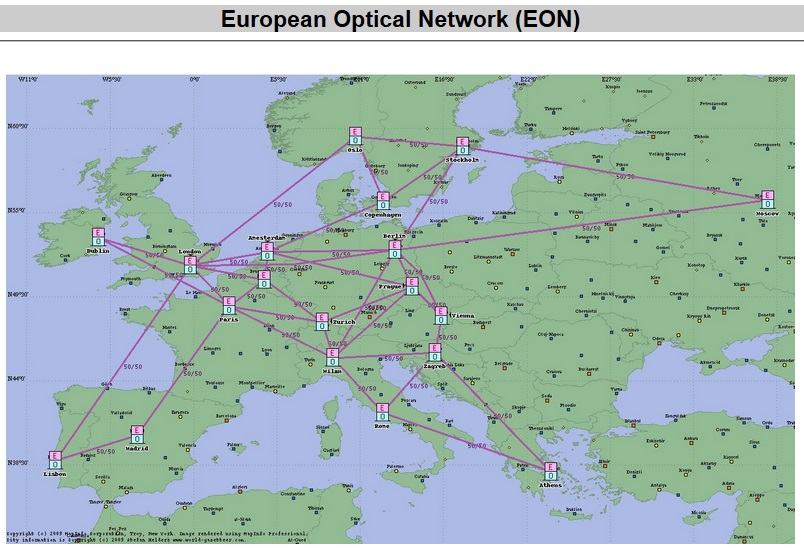
\includegraphics[width=\textwidth]{EON_Rede_Realista}
\caption{Physical topology of the realistic network.}
\end{figure}

The table \ref{table:2} shows the values of the variables associated with this network.
\begin{table}[h!]
\centering
\begin{tabular}{|| c | c | c||}
 \hline
 Constant & Description & Value \\
 \hline\hline
 N & Number of nodes & 19 \\
 L & Number of bidirectional links & 37 \\
 <$\delta$> & Node out-degree & 3.89 \\
 <len> & Mean link length (km) & 753.76 \\
 <h> & Mean number of hops for working paths & 2.3 \\
 <h'> & Mean number of hops for backup paths & 3.2 \\
 \hline
\end{tabular}
\caption{Table of realistic network values}
\label{table:2}
\end{table}

Again, through the ODU's we can calculate the total traffic for both scenarios being them:
\begin{itemize}
  \item Low Traffic: \textbf{2 TBits/s}
  \item High Traffic: \textbf{20 TBits/s}
\end{itemize}


\[
  \text{Dist} = \kbordermatrix{
    & Oslo & Stockholm & Moscow & Copenhagen & Berlin & Prague & Vienna & Zagreb & Athens & Rome & Milan & Zurich & Brussels & Amesterdan & London & Dublin & Paris & Madrid & Lisbon \\
    Oslo & 0 & 500 & 500 & 0 & 0 & 0 & 0 & 500 & 500 & 0 & 0 & 500 & 500 & 0 & 0 & 0 & 0 & 500 & 500 \\
    Stockholm & 0 & 500 & 500 & 0 & 0 & 0 & 0 & 500 & 500 & 0 & 0 & 500 & 500 & 0 & 0 & 0 & 0 & 500 & 500 \\
    Moscow & 0 & 500 & 500 & 0 & 0 & 0 & 0 & 500 & 500 & 0 & 0 & 500 & 500 & 0 & 0 & 0 & 0 & 500 & 500 \\
    Copenhagen & 0 & 500 & 500 & 0 & 0 & 0 & 0 & 500 & 500 & 0 & 0 & 500 & 500 & 0 & 0 & 0 & 0 & 500 & 500 \\
    Berlin & 0 & 500 & 500 & 0 & 0 & 0 & 0 & 500 & 500 & 0 & 0 & 500 & 500 & 0 & 0 & 0 & 0 & 500 & 500 \\
    Prague & 0 & 500 & 500 & 0 & 0 & 0 & 0 & 500 & 500 & 0 & 0 & 500 & 500 & 0 & 0 & 0 & 0 & 500 & 500 \\
    Vienna & 0 & 500 & 500 & 0 & 0 & 0 & 0 & 500 & 500 & 0 & 0 & 500 & 500 & 0 & 0 & 0 & 0 & 500 & 500 \\
    Zagreb & 0 & 500 & 500 & 0 & 0 & 0 & 0 & 500 & 500 & 0 & 0 & 500 & 500 & 0 & 0 & 0 & 0 & 500 & 500 \\
    Athens & 0 & 500 & 500 & 0 & 0 & 0 & 0 & 500 & 500 & 0 & 0 & 500 & 500 & 0 & 0 & 0 & 0 & 500 & 500 \\
    Rome & 0 & 500 & 500 & 0 & 0 & 0 & 0 & 500 & 500 & 0 & 0 & 500 & 500 & 0 & 0 & 0 & 0 & 500 & 500 \\
    Milan & 0 & 500 & 500 & 0 & 0 & 0 & 0 & 500 & 500 & 0 & 0 & 500 & 500 & 0 & 0 & 0 & 0 & 500 & 500 \\
    Zurich & 0 & 500 & 500 & 0 & 0 & 0 & 0 & 500 & 500 & 0 & 0 & 500 & 500 & 0 & 0 & 0 & 0 & 500 & 500 \\
    Brussels & 0 & 500 & 500 & 0 & 0 & 0 & 0 & 500 & 500 & 0 & 0 & 500 & 500 & 0 & 0 & 0 & 0 & 500 & 500 \\
    Amesterdan & 0 & 500 & 500 & 0 & 0 & 0 & 0 & 500 & 500 & 0 & 0 & 500 & 500 & 0 & 0 & 0 & 0 & 500 & 500 \\
    London & 0 & 500 & 500 & 0 & 0 & 0 & 0 & 500 & 500 & 0 & 0 & 500 & 500 & 0 & 0 & 0 & 0 & 500 & 500 \\
    Dublin & 0 & 500 & 500 & 0 & 0 & 0 & 0 & 500 & 500 & 0 & 0 & 500 & 500 & 0 & 0 & 0 & 0 & 500 & 500 \\
    Paris & 0 & 500 & 500 & 0 & 0 & 0 & 0 & 500 & 500 & 0 & 0 & 500 & 500 & 0 & 0 & 0 & 0 & 500 & 500\\
    Madrid & 0 & 500 & 500 & 0 & 0 & 0 & 0 & 500 & 500 & 0 & 0 & 500 & 500 & 0 & 0 & 0 & 0 & 500 & 500 \\
    Lisbon & 0 & 500 & 500 & 0 & 0 & 0 & 0 & 500 & 500 & 0 & 0 & 500 & 500 & 0 & 0 & 0 & 0 & 500 & 444
  }
\]


\newpage
\subsection{Dimensioning using ILP}
\begin{tcolorbox}	
\begin{tabular}{p{2.75cm} p{0.2cm} p{10.5cm}} 	
\textbf{Student Name}  &:& Tiago Esteves    (October 03, 2017 - )\\
\textbf{Goal}          &:& Implement the dimensioning of optical networks in the opaque transport mode.
\end{tabular}
\end{tcolorbox}

\subsubsection{ILP models}\label{ILP_models_OP}

For a better understanding of the functions and variables used in the ILP, a table \ref{description_opaque} will be created with all the variables and their description. \\

\begin{table}[h!]
\centering
\begin{tabular}{ |p{1cm}||p{13cm}|}
 \hline
 \multicolumn{2}{|c|}{Description of notation used in the objective function} \\
 \hline
 \hline
 $i$ & index for start node of a physical link \\
 $j$ & index for end node of a physical link \\
 $o$ & index for node that is origin of a demand \\
 $d$ & index for node that is destination of a demand \\
 $($ i,j $)$ & physical link between the nodes $i$ and $j$ \\
 $($ o,d $)$ & demand between the nodes $o$ and $d$ \\
 $c$ & index for bit rate of the client signal \\
 $C$ & set of the client signal \\
 $f_{ij}^{od}$ & binary variable indicating if link between the nodes $i$ and $j$ is used in the path between nodes $o$ and $d$ \\
 $W_{ij}$ & number of optical channels between the nodes $i$ and $j$\\
 $B_c $ & client signals granularities $($1.25, 2.5, 10, 40, 100$)$ \\
 $D_{odc}$ & client demands with bit rate $c$ between nodes $o$ and $d$ \\
 $G$ & network topology in form of adjacency matrix \\
 \hline
\end{tabular}
\caption{Table with description of variables}
\label{description_opaque}
\end{table}
\vspace{11pt}

The objective function of following ILP is a minimization of the sum of two variables: total number of flows crossing link (i,j) for all demand pairs (o,d) and total number of optical channels in each link (i,j).
\vspace{11pt}

\begin{equation}
minimize    \sum_{(i,j)} \sum_{(o,d)} f_{ij}^{od} + \sum_{(i,j)} W_{ij}
\label{ILPOpaque}
\end{equation}

\newpage
$subject$ $to$
\begin{equation}
\sum_{j\textbackslash \{o\}} f_{ij}^{od} = 2  \qquad \qquad \qquad \qquad \qquad \qquad \qquad \qquad \qquad \qquad
\forall(o,d) : o < d, \forall i: i = o
\label{ILPOpaque1}
\end{equation}

\vspace{-5pt}
\begin{equation}
\sum_{j\textbackslash \{o\}} f_{ij}^{od} = \sum_{j\textbackslash \{d\}} f_{ji}^{od}   \qquad \qquad \qquad \qquad \qquad \qquad \qquad \qquad
\forall(o,d) : o < d, \forall i: i \neq o,d
\label{ILPOpaque2}
\end{equation}

\begin{equation}
\sum_{j\textbackslash \{d\}} f_{ji}^{od} = 2  \qquad \qquad \qquad \qquad \qquad \qquad \qquad \qquad \qquad \qquad
\forall(o,d) : o < d, \forall i: i = d
\label{ILPOpaque3}
\end{equation}

\begin{equation}
\sum_{(o,d):o<d} \left(f_{ij}^{od} + f_{ji}^{od}\right) + \sum_{c\in C} (B\left(c\right) D_{cod}\leq100 W_{ij} G_{ij} \qquad \qquad \qquad \qquad \qquad
\forall(i,j) : i < j
\label{ILPOpaque4}
\end{equation}

\begin{equation}
W_{ij} \leq 80 \qquad  \qquad \qquad \qquad \qquad \qquad \qquad \qquad \qquad \qquad \qquad \qquad \qquad \forall(i,j) : i < j
\label{ILPOpaque5}
\end{equation}

\begin{equation}
f_{ij}^{od} , f_{ji}^{od} \in \{0,2\}   \qquad \qquad \qquad \qquad \qquad \qquad \qquad \qquad \qquad
\forall(i,j) : i < j, \forall(o,d) : o < d
\label{ILPOpaque6}
\end{equation}

\begin{equation}
W_{ij} \in \mathbb{N}  \qquad \qquad \qquad \qquad \qquad \qquad \qquad \qquad \qquad \qquad \qquad \qquad \qquad
\forall(i,j) : i < j\label{ILPOpaque7}
\end{equation}

\vspace{10pt}

The objective function, to be minimized, is the expression \ref{ILPOpaque}. The flow conservation constraints are \ref{ILPOpaque1}, \ref{ILPOpaque2} and \ref{ILPOpaque3}. First constraint ensures that, for all demand pairs (o,d), it routes two flows of traffic for all bidirectional links (i,j) when $j$ is not equal to the origin of the demand. Equation \ref{ILPOpaque3} is based on the same idea of \ref{ILPOpaque}, however applied in reverse direction. Assuming bidirectional traffic, so the number of flows in both directions of the link is the same \ref{ILPOpaque2}. The inequality \ref{ILPOpaque4} is considered grooming constraint, so it means the total client traffic flows can not be greater than the capacity of optical channels on all links. Another important constraint \ref{ILPOpaque5} is the capacity of the optical channels which must be less or equal to 100 Gb/s or 80 ODU0. The number of flows per demand can be zero if there are no traffic demands or two if considering working and protection traffic \ref{ILPOpaque6}. The last constraint \ref{ILPOpaque7} is just needed to ensure the number optical of channels is a positive integer values greater than zero.

\subsubsection{ILP Results}

In this initial phase the results will be presented using ILP to calculate the CAPEX of the reference network and the realistic network.
The value of the CAPEX of the network will be calculated based on the costs of the equipment present in the table below.

\begin{table}[h!]
\centering
\begin{tabular}{|| c | c||}
 \hline
 Equipment & Cost \\
 \hline\hline
 OLT without transponders & 15000 \euro \\
 Transponder & 5000 \euro/Gb \\
 Optical Amplifier & 4000 \euro \\
 EXC & 10000 \euro \\
 OXC & 20000 \euro \\
 EXC Port & 1000 \euro /Gb/s\\
 OXC Port & 2500 \euro /porto \\
 \hline
\end{tabular}
\caption{Table with costs}
\label{table_cost1}
\end{table}

In addition to the equipment costs we will also use the parameter "span", which in this case will have a value of 100, because this value is used to calculate the number of optical amplifiers required in the network using Equation \ref{amplifiers}.

\begin{equation}
N^R = \sum\limits_{l=1}^L\left(\left\lceil\frac{len_l}{span}\right\rceil-1\right)
\label{amplifiers}
\end{equation}

The other parameters of this equation are:
\begin{itemize}
\item{$N^R$			$\rightarrow$ Total number of regenerators/amplifiers}
\item{$len_l$		$\rightarrow$ Length of link l}
\item{$span$		$\rightarrow$ Distance between amplifiers}	
\end{itemize}	

To know the value of CAPEX it is necessary to know the value of the cost of the links and the cost of the nodes.
To calculate the cost of the nodes, the sum of the costs of the optical and electrical node is made. For this case the value of the optical cost is zero only needing to know the electric cost of the nodes that is given by equation \ref{electricalCostOpaque}.

\begin{equation}
C_{exc} = \left(\gamma_{e0}\times N\right) + \gamma_{e1} \times \left(T_1 + \left(2 \times w^0 \times \tau \right)\right)
\label{electricalCostOpaque}
\end{equation}

\begin{itemize}
\item{$C_{exc}$		$\rightarrow$	Electrical ports cost}
\item{$\gamma_{e0}$	$\rightarrow$	EXC cost in euros}
\item{$N$			$\rightarrow$	Number of nodes}
\item{$\gamma_{e1}$	$\rightarrow$	EXC port cost in euros}
\item{$T_1$         $\rightarrow$   Total unidirectional traffic}
\item{$w^0$			$\rightarrow$	Total number of optical channels}
\item{$\tau$		$\rightarrow$	Traffic per port}
\end{itemize}

To calculate the cost of the Links we will use the equation \ref{linkCosts}.

\begin{equation}
C_L = \left(2 \times \gamma_0^{OLT} \times L\right) + \left(2 \times \gamma_1^{OLT} \times \tau \times W\right) + \left(N^R \times c^R\right)
\label{linkCosts}
\end{equation}	
	
\begin{itemize}
\item{$C_L$				$\rightarrow$	Links cost}
\item{$\gamma_0^{OLT}$	$\rightarrow$	OLT cost in euros}
\item{$L$				$\rightarrow$	Number of unidirectional links}
\item{$\gamma_1^{OLT}$	$\rightarrow$	Transponder cost in euros}
\item{$W$             $\rightarrow$	    Total number of optical channels}
\item{$N^R$				$\rightarrow$	Total number of optical amplifiers}
\item{$c^R$				$\rightarrow$	Optical amplifiers cost in euros}
\end{itemize}

\vspace{11pt}
To perform the calculations using the implementation of the models described in section \ref{ILP_models_OP} it is necessary to use a mathematical software tool. For this we will use MATLAB which is ideal for dealing with linear programming problems and can call the LPsolve through an external interface. \\

\textbf{Scenario 1: Test Network Low Traffic} \label{Scenario1_opaque} \\
In this scenario we used the table \ref{table:1}. In the table \ref{result_ILP1} we can see the values calculated through MatLab and using the values indicated in table \ref{table_cost1} we can finally calculate the CAPEX value. \\

\begin{table}[h!]
\centering
\begin{tabular}{|| c | c||}
 \hline
 Number of optical channels & Value \\
 \hline\hline
 in the link (1,2) & 2 \\
 in the link (1,3) & 2 \\
 in the link (2,3) & 4 \\
 in the link (2,4) & 3 \\
 in the link (3,5) & 3 \\
 in the link (4,5) & 3 \\
 in the link (4,6) & 3 \\
 in the link (5,6) & 3 \\
 \hline
\end{tabular}
\caption{Table with results}
\label{result_ILP1}
\end{table}


Using equation \ref{linkCosts} : \\
$C_L$ = $($2 * 15 000 * 8$)$ + $($2 * 5 000 * 100 * 23$)$ + $($24 * 4 000$)$ \\
$C_L$ = \textbf{23 336 000\euro} \\
\newpage
Using equation \ref{electricalCostOpaque} : \\
$C_{exc}$ = $($6 * 10 000$)$ + 1 000 * $($1 000 + $($2 * 23 * 100$)$ $)$ \\
$C_N$ = $C_{exc}$ = \textbf{5 660 000\euro} \\

$CAPEX$ = 23 336 000 + 5 660 000 = \textbf{28 996 000\euro}\\


\vspace{11pt}
\textbf{Scenario 2: Test Network High Traffic} \label{Scenario2_opaque} \\
In this scenario we used again the table \ref{table:1}. In the table \ref{result_ILP2} we can see the values calculated through MatLab and using the values indicated in table \ref{table_cost1} we can finally calculate the CAPEX value. \\

\begin{table}[h!]
\centering
\begin{tabular}{|| c | c||}
 \hline
 Number of optical channels & Value \\
 \hline\hline
 in the link (1,2) & 6 \\
 in the link (1,3) & 6 \\
 in the link (2,3) & 17 \\
 in the link (2,4) & 14 \\
 in the link (3,5) & 14 \\
 in the link (4,5) & 13 \\
 in the link (4,6) & 15 \\
 in the link (5,6) & 15 \\
 \hline
\end{tabular}
\caption{Table with results}
\label{result_ILP2}
\end{table}


Using equation \ref{linkCosts} : \\
$C_L$ = $($2 * 15 000 * 8$)$ + $($2 * 5 000 * 100 * 100$)$ + $($24 * 4 000$)$ \\
$C_L$ = \textbf{100 336 000\euro} \\

Using equation \ref{electricalCostOpaque} : \\
$C_{exc}$ = $($6 * 10 000$)$ + 1 000 * $($1 000 + $($2 * 100 * 100$)$ $)$ \\
$C_N$ = $C_{exc}$ = \textbf{21 060 000\euro} \\

$CAPEX$ = 100 336 000 + 21 060 000 = \textbf{121 396 000\euro}\\


\vspace{11pt}
\textbf{Scenario 3: Realistic Network Low Traffic} \label{Scenario3_opaque} \\
In this scenario we used the table \ref{table:2}. In the table \ref{result_ILP1} we can see the values calculated through MatLab and using the values indicated in table \ref{table_cost3} we can finally calculate the CAPEX value. \\
\newpage
\begin{table}[h!]
\centering
\begin{tabular}{|| c | c||}
 \hline
 Number of optical channels & Value \\
 \hline\hline
 in the link (1,2) &  \\
 in the link (1,3) &  \\
 in the link (2,3) &  \\
 in the link (2,4) &  \\
 in the link (3,5) &  \\
 in the link (4,5) &  \\
 in the link (4,6) &  \\
 in the link (5,6) &  \\
 \hline
\end{tabular}
\caption{Table with results}
\label{result_ILP3}
\end{table}


Using equation \ref{linkCosts} : \\
$C_L$ = $($2 * 15 000 * 37$)$ + $($2 * 5 000 * 100 * $)$ + $($24 * 4 000$)$ \\
$C_L$ = \textbf{ \euro} \\

Using equation \ref{electricalCostOpaque} : \\
$C_{exc}$ = $($19 * 10 000$)$ + 1 000 * $($1 000 + $($2 *  * 100$)$ $)$ \\
$C_N$ = $C_{exc}$ = \textbf{ \euro} \\

$CAPEX$ =  +  = \textbf{ \euro}\\


\vspace{11pt}
\textbf{Scenario 4: Realistic Network High Traffic} \label{Scenario4_opaque} \\
In this scenario we used again the table \ref{table:2}. In the table \ref{result_ILP4} we can see the values calculated through MatLab and using the values indicated in table \ref{table_cost1} we can finally calculate the CAPEX value. \\

\begin{table}[h!]
\centering
\begin{tabular}{|| c | c||}
 \hline
 Number of optical channels & Value \\
 \hline\hline
 in the link (1,2) &  \\
 in the link (1,3) &  \\
 in the link (2,3) &  \\
 in the link (2,4) &  \\
 in the link (3,5) &  \\
 in the link (4,5) &  \\
 in the link (4,6) &  \\
 in the link (5,6) &  \\
 \hline
\end{tabular}
\caption{Table with results}
\label{result_ILP4}
\end{table}


Using equation \ref{linkCosts} : \\
$C_L$ = $($2 * 15 000 * 37$)$ + $($2 * 5 000 * 100 * $)$ + $($24 * 4 000$)$ \\
$C_L$ = \textbf{ \euro} \\

Using equation \ref{electricalCostOpaque} : \\
$C_{exc}$ = $($19 * 10 000$)$ + 1 000 * $($1 000 + $($2 * 100 * $)$ $)$ \\
$C_N$ = $C_{exc}$ = \textbf{\euro} \\

$CAPEX$ =  +  = \textbf{\euro}\\

\newpage

\subsection{Dimensioning using Heuristics}

\subsubsection{Heuristics Models}

\subsubsection{Heuristics Results}

\subsection{Comparative Analysis}
